\input{../../input/main}

\usetikzlibrary{hobby}

\begin{document}

\begin{center}
  \Large{\textbf{Городской центр физического образования, 10 класс.}\\
  \textit{Серия 9, 20 ноября 2014.}}
\end{center}

\begin{center}
  \Large \textbf{ Районный тур уже близко: механика. }
\end{center}

\large

\task{ По вертикальному длинному стержню могут без трения двигаться
  две маленькие бусинки. Бусинки упруго соударяются друг с другом, а
  нижняя упруго соударяется с землёй. Бусинки запустили так, что
  верхняя, которая в $n=104$ раза тяжелее нижней, практически
  неподвижно зависла на высоте $H=1$ м над землей. Оцените скорость,
  которую в среднем имеет нижняя бусинка у земли. Ускорение свободного
  падения $g = 9,8 \mbox{ м/с}^2$. }
% СПб, город-10, 2001

\taskpic{ Наклонная плоскость расположена под углом $\alpha$ к
  горизонту. В начальный момент тело находится в точке
  \textbf{A}. Выше вдоль плоскости на $h$ и правее на $l$, в точке
  \textbf{B}, располагается лунка. Какую начальную скорость $V$ под
  углом $\beta$ к горизонтали надо придать телу вдоль плоскости, чтобы
  оно попало в лунку, скользя без трения? Ускорение свободного падения
  $g$. }
{
  \begin{tikzpicture}
    \draw[thick] (0,0) -- (2,0);
    \draw[thick] (2,0) -- ++(40:2cm) -- ++(0,1) -- (2,0);
    \draw[thick] (2,0) ++(40:2cm) ++ (0,1) -- ++(-2,0) -- (0,0);
    \draw[thick,dashed] (0,0) ++(45:1.5cm) -- ++(1.2,0);
    \draw[very thick,->] (0,0) ++(45:1.5cm) node[below] {\textbf{A}} --
    ++(40:1cm); 
    \draw[fill=black] (0,0) ++(35:2.8cm) circle (0.05cm) node[above
    right] {\textbf{B}};
    \draw[blue,thick,->] (2,3) node[left] {$\beta$} to[out=0,in=20]
    ($(0,0)+(42:1.7cm)$);
    \draw[blue,thick,->] (0,0) ++(5:3cm) node[below] {$\alpha$}
    to[out=90,in=20] (2.4,0.5);  
  \end{tikzpicture}
}
% СПб, город-11, 2007

\task{ На длинный горизонтальный стержень надеты $N$ одинаковых
  неупругих бусинок. С краю находится еще одна бусинка в 2 раза
  большей массы. Ей придают некоторую скорость в направлении остальных
  бусинок, сообщая кинетическую энергию $E$. Найдите выделившееся в
  результате соударений тепло. Трением пренебречь. }

\taskpic{ Незадачливые артиллеристы стреляют из пушки, стоящей на
  наклонной плоскости. В момент выстрела пушка срывается с креплений и
  начинает соскальзывать вниз с нулевой начальной скоростью. Ядро
  вылетает и попадает в соскальзывающую пушку. Коэффициент трения
  скольжения пушки о плоскость равен $\mu$. Пренебрегая сопротивлением
  воздуха, определите под каким углом к наклонной плоскости вылетело
  ядро из пушки. }
{
  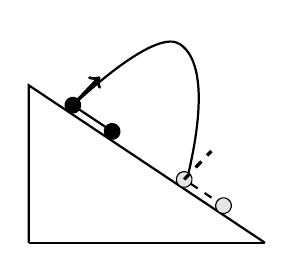
\begin{tikzpicture}
    \draw[thick] (0,0) -- (3,0);
    \draw[thick] (0,0) -- ++(0,2) -- (3,0);
    \begin{scope}[rotate around={{-atan(2/3)}:(3,0)}]
      \draw[fill=black] (0,0.1) circle (0.1cm);
      \draw[thick] (0.1,0.1) -- ++(0.5,0);
      \draw[fill=black] (0.6,0.1) circle (0.1cm);
      \draw[very thick,->] (0,0.1) -- ++(80:0.5cm);
      \draw[thick] (0,0.1) parabola bend (0.7,1.5) (1.7,0.2); 
    \end{scope}
    \begin{scope}[rotate around={{-atan(2/3)}:(3,0)},xshift=1.7cm]
      \draw[fill=gray!20] (0,0.1) circle (0.1cm);
      \draw[thick,dashed] (0.1,0.1) -- ++(0.5,0);
      \draw[fill=gray!20] (0.6,0.1) circle (0.1cm);
      \draw[very thick,dashed] (0,0.1) -- ++(80:0.5cm); 
    \end{scope}
  \end{tikzpicture}
}
% СПб, город-10, 2009

\end{document}


%%% Local Variables: 
%%% mode: latex
%%% TeX-engine:xetex
%%% TeX-PDF-mode: t
%%% End:
